\documentclass[10pt, a4paper]{beamer}
\usetheme{metropolis}           % Use metropolis theme
\usepackage[utf8]{inputenc}
\usepackage{amsmath,amsfonts,amssymb}
\usepackage{dsfont}
\usepackage{graphicx}
\usepackage{caption}


\title{Wigner's Semicircle Law}
\date{\today}
\author{Sacha Ben-Arous}
\institute{ENS Paris-Saclay}
\begin{document}
  \maketitle
  
\begin{frame}
\tableofcontents
\end{frame}  

\section{Universality in Probability Theory}

\begin{frame}{First theorems}
    Two fundamentals theorems :
\begin{itemize}
\item <1> \only<1>{\textbf{Law of Large Numbers : } $(X_i)_{i \in \mathbb{N}^*}$ an infinite sequence of \textit{i.i.d}, \textit{Lebesgue integrable} random variables where $\begin{cases} \mu := \mathbb{E}[X_1]\\ \overline{X_n} := \frac{1}{n}(X_1 + \dots X_n) \end{cases}$ \[ \overline{X_n} \xrightarrow{\mathbb{P}} \mu \]}
\item <2> \only<2>{\textbf{Central Limit Theorem : } $(X_i)_{i \in \mathbb{N}^*}$ an infinite sequence of \textit{i.i.d} random variables with \textit{finite variance} where $\begin{cases} \mu := \mathbb{E}[X_1] \\ \sigma := \mathbb{E}[(X_1-\mu)^2] \\ \overline{X_n} := \frac{1}{n}(X_1 + \dots X_n) \end{cases}$ 
\[ \sqrt{n}(\overline{X_n}-\mu) \xrightarrow{\mathcal{L}} \mathcal{N}(0,\sigma^2) \]}
\end{itemize}
\end{frame}

\begin{frame}{Universality}
In both of the previous theorems, the probability distribution of the $(X_i)_{i \in \mathbb{N}}$ does not affect the limit results. Therefore, these laws are described as \textbf{universal}, meaning the can be applied for every random sample of independant experiments.
\end{frame}

\section{Wigner's Law}

\begin{frame}{History}
First studied by Wishart in the 1920s, then by Wigner in the case of a physics problem : Wigner studied the interactions between atoms, which can be described using linear operators. Therefore, the behavior of the eigenvalues of those operators was crucial (ex: PCA), but almost impossible to compute. Wigner's idea was to consider random matrices that were 
similar to the ones describing atoms interactions, but whose eigenvalues were easier to study.
\end{frame}

\begin{frame}{Notations}
\only<1>{We consider an infinite family of \textit{i.i.d}, random variables$(W_{i,j})_{i,j \in \mathbb{N}} $ that verifies the following properties : $\begin{cases} \forall i,j \ W_{i,j}=W_{j,i} \\ \mathbb{E}(W_{1,1})=0 \\ \mathbb{E}\left (\left| W_{1,1}  \right|^2\right )=1 \\ \forall k \geq 3 $, $ \mathbb{E}(\left| W_{1,1}  \right|^k) < +\infty \end{cases}$}
\only<2>{Then, we consider $W_n := (W_{i,j})_{1 \leq i,j \leq n}$. Because $W_n$ is symmetric, it has exactly $n$ eigenvalues. Therefore, we denote : $\text{SP}(\frac{W_n}{\sqrt{n}})= \{ \lambda_i , i \in \{1,\dots,n\}\} $.\\}

\end{frame}

\begin{frame}{Theorem}
\textbf{Wigner's Law : } For every "reasonable" function $f$ : 
\[ \lim_{n \to \infty} \mathbb{E}\left (\frac{1}{n} \sum_{i=1}^n f(\lambda_i)\right ) = \int_{-2}^2 f(x) \, \mathrm{d}\mu_{SC}^{(\sigma)}(x) \] where $\mathrm{d}\mu_{SC}$ is the density of the semi-cercle of radius $2\sigma$, centered in $0$, given by  : \[ \mathrm{d}\mu_{SC}^{(\sigma)}(x) =\frac{1}{2\pi{\sigma^2}}\mathds{1}_{[-2;2]}(x)\sqrt{4\sigma^2-x^2} \mathrm{d}x \]

Ex : $f$ can be a continous and bouded function, or an indicator function.
\end{frame}

\begin{frame}{Explanation}
\only<1>{One way of seeing the link with a semi-circle is to apply the theorem with $f$ and indicator function of the set $[-\infty;a]$, where $a \in [-2;2]$ :
\[\lim_{n \to \infty} \mathbb{E}\left (\frac{1}{n} \sum_{i=1}^n \mathds{1}_{[-\infty;a]}(\lambda_i)\right ) = \int_{-2}^2 \mathds{1}_{[-\infty;a]}(x) \, \mathrm{d}\mu_{SC} \]
Thus \[\lim_{n \to \infty} \mathbb{E}\left (\frac{|\{i, \lambda_i \leq a \}|}{n}\right )=\int_{-\infty}^a \mathrm{d}\mu_{SC}\]
Therefore, the limit density of the $(\lambda_i)_{i \in \mathbb{N}}$ is given by the semi-circle density.}
\only<2>{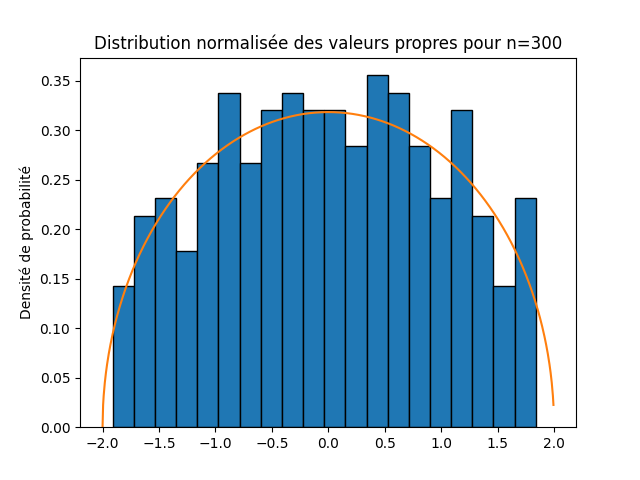
\includegraphics[scale=0.29]{Figure_300.png} 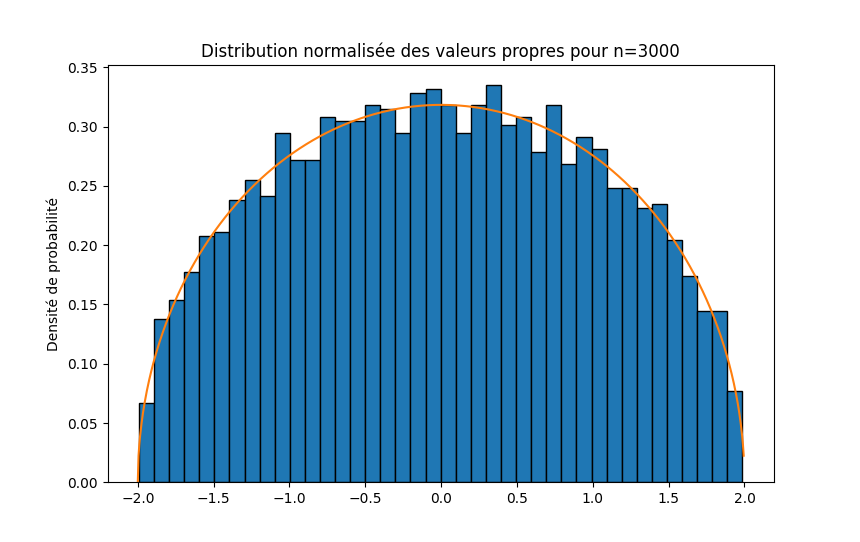
\includegraphics[scale=0.27]{Figure_1.png}
\captionof{figure}{Exemple where $W_{1,1}$ follows a Rademacher law}}
\end{frame}

\section{Sketch of the proof}

\begin{frame}{Idea}
The main idea of the proof is to reduce the problem to the exponent functions : $x \mapsto x^k $. Then, using density theorems such as Weierstrass theorem, we could easily generalize to continous bounded function on intervals. Finally, limiting the maximum eigenvalue will give the general case.
\end{frame}

\begin{frame}{Proof}
\only<1>{Our goal is to show that :  $ \mathbb{E}\left (\frac{1}{n} \sum_{i=1}^n \lambda_i^k\right ) = \int_{-2}^{2} x^{k} \, \mathrm{d}\mu_{SC}  $}
\only<2>{We need to study the following quantity : 
\begin{eqnarray*}
\mathbb{E}\left (\frac{1}{n} \sum_{i=1}^n \lambda_i^k\right )&=&\mathbb{E}\left (\frac{1}{n}\text{Tr}\left (\left (\frac{W_n}{\sqrt{n}}\right )^k\right )\right )\\
&=&\sum_{i_1,\dots,i_k=1}^n n^{-\frac{k}{2}-1}\mathbb{E}[(W_n)_{i_1,i_2}\dots(W_n)_{i_k,i_1}] \\
&=&\sum_{I \in \{1,\dots,n\}^k} n^{-\frac{k}{2}-1}P(I)\end{eqnarray*}
where if $I=(i_1,\dots,i_k) \in \{1,\dots,n\}^k $ then $P(I):=\mathbb{E}[(W_n)_{i_1,i_2}\dots(W_n)_{i_k,i_1}]$.}
\only<3>{The technique to use is the following : if there is too much different values in $I$, because $(W_{i,j})_{i,j \in \mathbb{N}}$ are independant, we will be able to extract one $\mathbb{E}[(W_n)_{i,j}]$, making $P(I)$ equal to $0$ because of the assumptions. Next, the set of $I$ that contains a 'small' amout of values has a negligible size, therefore it will not contribute to the final sum. Therefore, the only terms contributing to the final value are the ones between these two cases.}
\only<4>{\textbf{Lemma 1 :} The important cases is reached for the $I$ such that the number of distinct values in I is $\frac{k}{2}$. \\ 

\textbf{Lemma 2 :}
  $ \begin{cases}\lim_{n \to \infty} \mathbb{E}\left (\frac{1}{n} \sum_{i=1}^n \lambda_i^{2q}\right ) = \text{Cat}(q) \\ \lim_{n \to \infty} \mathbb{E}\left (\frac{1}{n} \sum_{i=1}^n \lambda_i^{2q+1}\right ) = 0 \end{cases}$ }
\end{frame}

\section{What comes next ?}

\begin{frame}{More precision}

\only<1>{As seen in the first slides, we can now wonder what is the error of our theorem by looking at the extreme eigenvalue. It's evolution is given by the Tracy-Widom law : 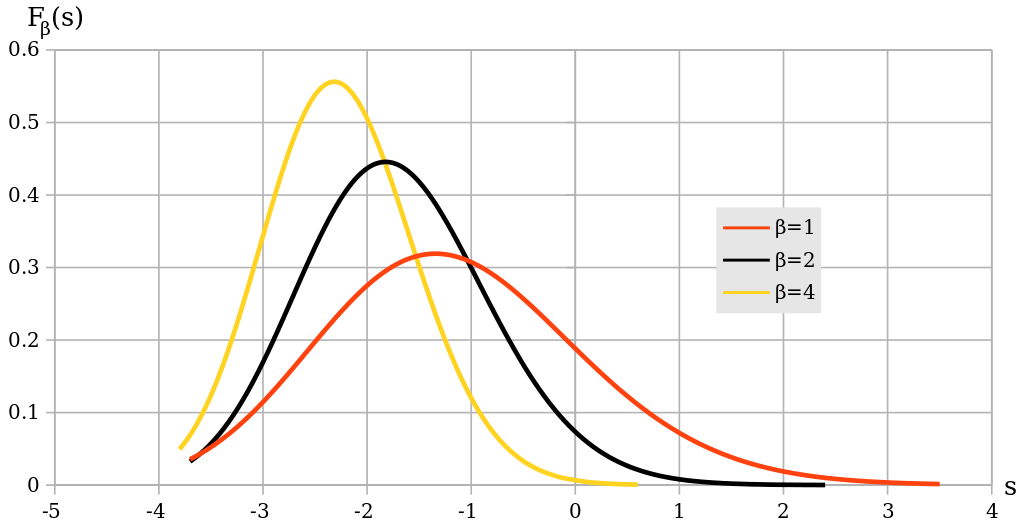
\includegraphics[scale=0.25]{TracyWidom.png}}
\only<2>{In the "bulk", the behavior of the eigenvalues is well-known, with an average space between two consecutive eigenvalues of $\frac{1}{n}$}

\end{frame}


\begin{frame}{Questions}

Any questions ?

\end{frame}


\end{document}